% Asset ID: A22StatisticalHypothesisTestingTIKZ-003
% Unit code: A22
% Topic code: A22-HT
% Topic name: Statistical hypothesis testing
% Related lesson section: Core Theory, Critical value method for correlation tests
% Source: CCEA specification map; lesson transcript; Stats Yr2 Chapter 1 PDF
% Purpose: Provide a printable decision flowchart for correlation hypothesis tests.
% Status: Phase 4 TikZ draft

\documentclass[tikz,border=8pt]{standalone}
\usepackage{amsmath}
\usepackage{tikz}
\usetikzlibrary{arrows.meta, positioning, shapes.geometric}
\begin{document}
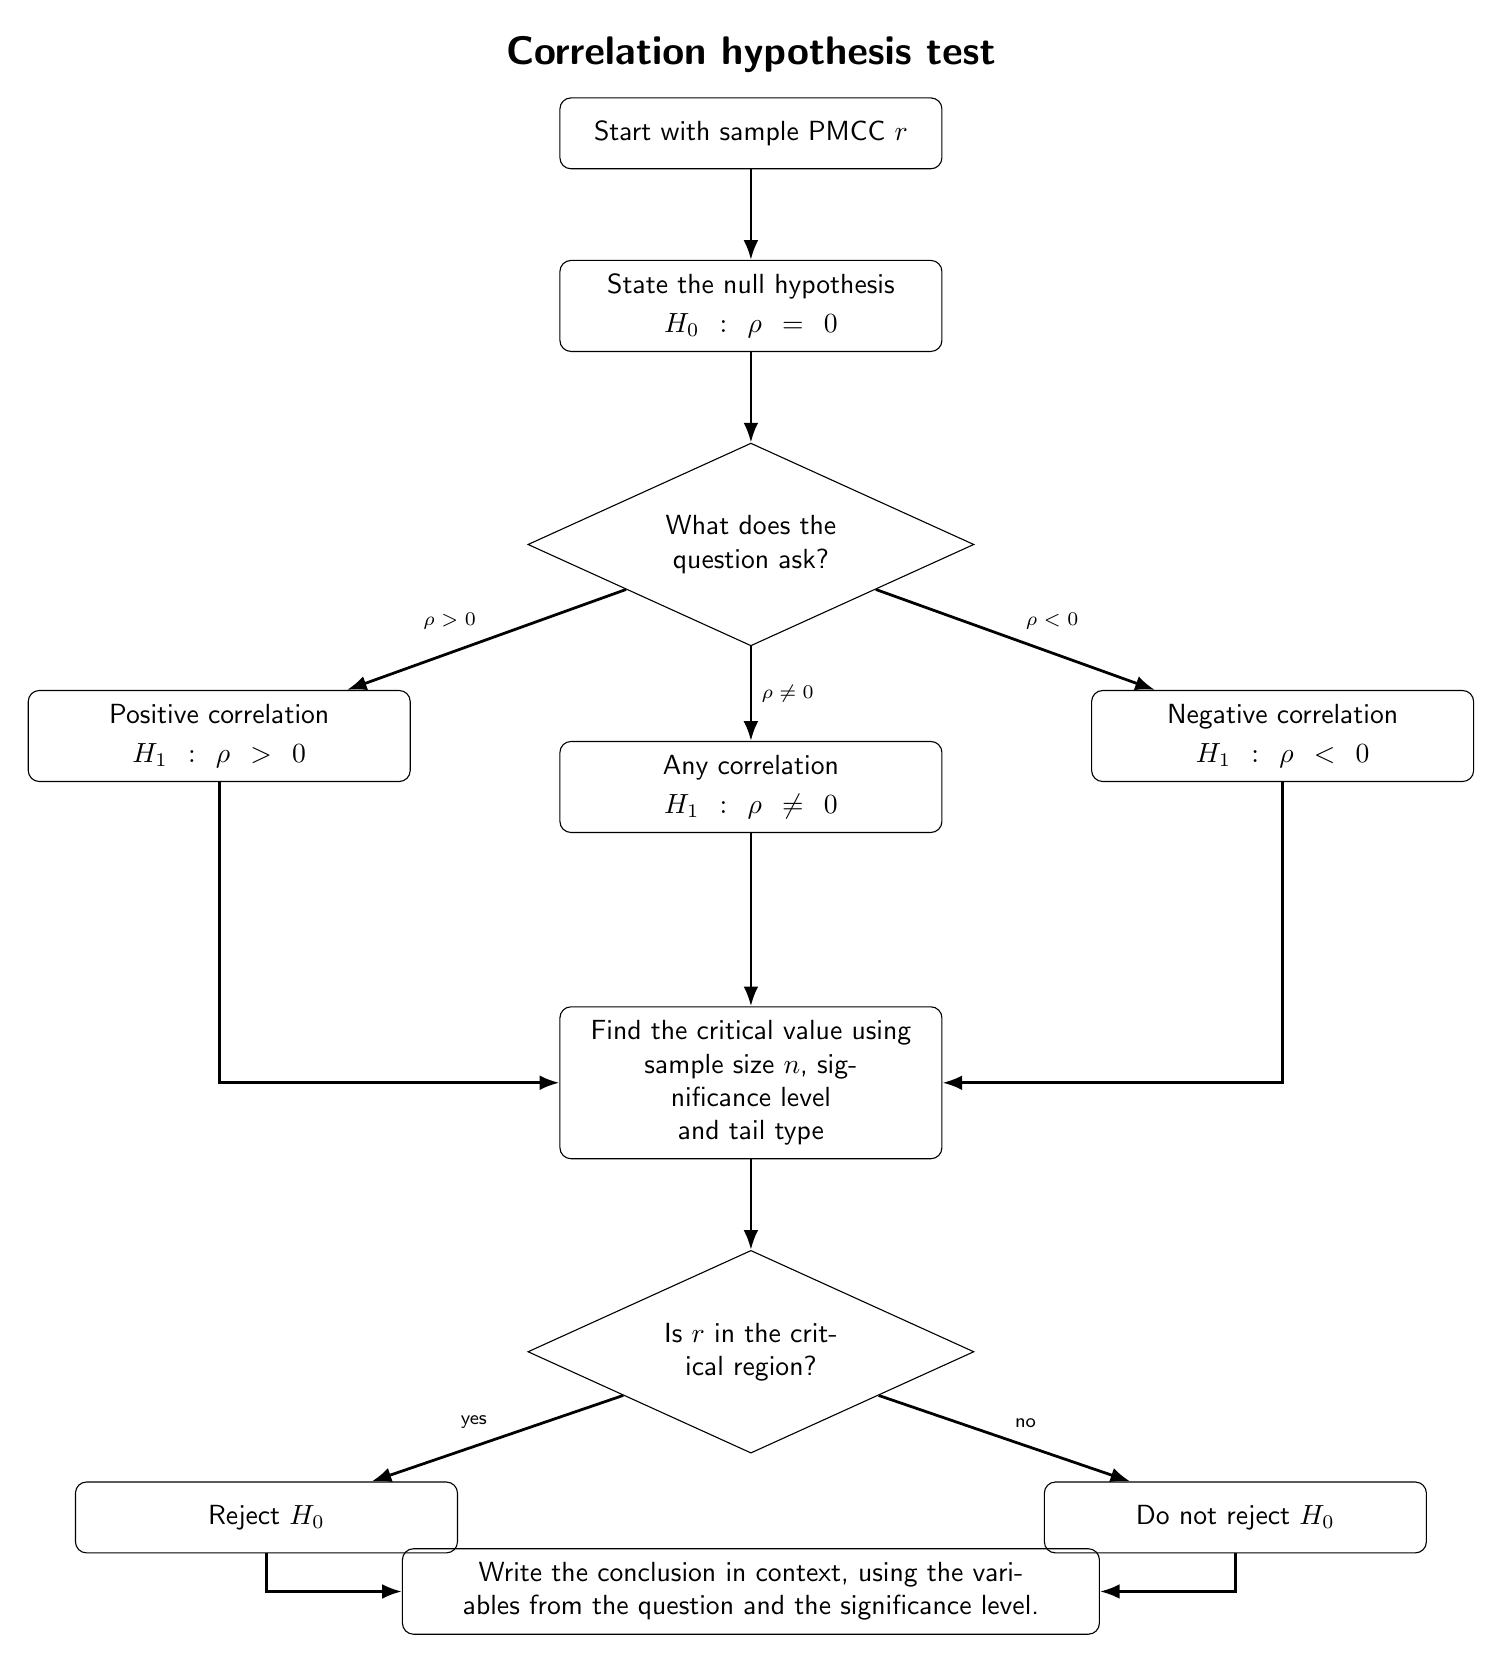
\begin{tikzpicture}[font=\sffamily,node distance=1.15cm,box/.style={draw,rounded corners=4pt,align=center,text width=4.5cm,minimum height=0.9cm,inner sep=5pt},decision/.style={draw,diamond,aspect=2.2,align=center,text width=3.6cm,inner sep=2pt},arrow/.style={line width=1pt,-{Latex[length=2.5mm]}}]
\node[font=\sffamily\bfseries\Large] (title) at (0,6.2){Correlation hypothesis test};
\node[box] (start) at (0,5.2){Start with sample PMCC \(r\)};
\node[box, below=of start] (h0){State the null hypothesis\\[2pt]\(\displaystyle H_0:\rho=0\)};
\node[decision, below=of h0] (wording){What does the question ask?};
\node[box, below left=1.2cm and 2.9cm of wording] (pos){Positive correlation\\[2pt]\(\displaystyle H_1:\rho>0\)};
\node[box, below=1.2cm of wording] (any){Any correlation\\[2pt]\(\displaystyle H_1:\rho\neq0\)};
\node[box, below right=1.2cm and 2.9cm of wording] (neg){Negative correlation\\[2pt]\(\displaystyle H_1:\rho<0\)};
\node[box, below=2.2cm of any] (crit){Find the critical value using\\sample size \(n\), significance level\\and tail type};
\node[decision, below=of crit] (compare){Is \(r\) in the critical region?};
\node[box, below left=1.0cm and 2.3cm of compare] (reject){Reject \(H_0\)};
\node[box, below right=1.0cm and 2.3cm of compare] (notreject){Do not reject \(H_0\)};
\node[box, below=1.2cm of compare, text width=8.5cm] (context){Write the conclusion in context, using the variables from the question and the significance level.};
\draw[arrow] (start) -- (h0); \draw[arrow] (h0) -- (wording); \draw[arrow] (wording) -- node[above left] {\scriptsize \(\rho>0\)} (pos); \draw[arrow] (wording) -- node[right] {\scriptsize \(\rho\neq0\)} (any); \draw[arrow] (wording) -- node[above right] {\scriptsize \(\rho<0\)} (neg); \draw[arrow] (pos) |- (crit); \draw[arrow] (any) -- (crit); \draw[arrow] (neg) |- (crit); \draw[arrow] (crit) -- (compare); \draw[arrow] (compare) -- node[above left] {\scriptsize yes} (reject); \draw[arrow] (compare) -- node[above right] {\scriptsize no} (notreject); \draw[arrow] (reject) |- (context); \draw[arrow] (notreject) |- (context);
\end{tikzpicture}
\end{document}
